\documentclass[conference]{IEEEtran}
\IEEEoverridecommandlockouts
% The preceding line is only needed to identify funding in the first footnote. If that is unneeded, please comment it out.
\usepackage{cite}
\usepackage{amsmath,amssymb,amsfonts}
\usepackage{algorithmic}
\usepackage{graphicx}
\usepackage{textcomp}
\usepackage{xcolor}
\usepackage{array}
\usepackage{stfloats}
\usepackage{pifont}

\usepackage[noblocks]{authblk}

\usepackage{algorithm}
%\usepackage[ruled,linesnumbered]{algorithm2e} 
%\usepackage{algpseudocode} 
%\usepackage{algorithmicx}    
\renewcommand{\algorithmicrequire}{\textbf{Input:}}  % Use Input in the format of Algorithm
\renewcommand{\algorithmicensure}{\textbf{Output:}} % Use Output in the format of Algorithm 

%缩进提示线





\def\BibTeX{{\rm B\kern-.05em{\sc i\kern-.025em b}\kern-.08em
		T\kern-.1667em\lower.7ex\hbox{E}\kern-.125emX}}

\begin{document}
	
	\title{
		%{\footnotesize}
		%\thanks{Identify applicable funding agency here. If none, delete this.}
	}
	
	\author[ ]{Xiang Chen}
	\author[ ]{Cailian Chen}
	\affil[ ]{Department of Automation, Shanghai Jiao Tong University, Shanghai 200240, P. R. China \authorcr Key Laboratory of System Control and Information Processing, Ministry of Education of China}
	\affil[*]{Corresponding Author. Email:Chen\_Xiang@sjtu.edu.cn}
	
	%\author{\IEEEauthorblockN{1\textsuperscript{st} Yunzhu Yu}
	%\IEEEauthorblockA{\textit{dept. name of organization (of Aff.)} \\
	%\textit{name of organization (of Aff.)}\\
	%Shanghai, China \\
	%YuYunzhu@sjtu.edu.cn}
	%\and
	%\IEEEauthorblockN{2\textsuperscript{nd} Kaijie Wu}
	%\IEEEauthorblockA{\textit{dept. name of organization (of Aff.)} \\
	%\textit{name of organization (of Aff.)}\\
	%Shanghai, China \\
	%email address or ORCID}
	%\and
	%\IEEEauthorblockN{3\textsuperscript{rd} Given Name Surname}
	%\IEEEauthorblockA{\textit{dept. name of organization (of Aff.)} \\
	%\textit{name of organization (of Aff.)}\\
	%City, Country \\
	%email address or ORCID}
	%}
	
	\maketitle
	
	\begin{abstract}
		
	\end{abstract}
	
	\begin{IEEEkeywords}
		Clock synchronization, Time sensitive networking, Precision time protocol (PTP), AS6802
	\end{IEEEkeywords}
	
	\section{Introduction}
	Many modern control strategies are time-triggered, and control systems are mostly distributed, so precise synchronization and time-deterministic communication are required.
	Time Sensitive Networking (TSN) is currently the most promising time deterministic communication method in industrial Ethernet applications. In the future, TSN will replace or extend most current industrial fieldbuses with its unified communication paradigm.
	Since wired-only networks cannot scale with a large number of nodes in a large automation project, hybrid solutions with wired backbone networks and multiple smaller wireless islands are considered(fig1). 
	\begin{figure}[htbp]	
		\centerline{\includegraphics[scale=0.5]{fig2.eps}}
		\caption{Heterogeneous network clock synchronization architecture.}
		\label{fig1}
	\end{figure}
	In these hybrid architectures, the wireless part should meet the same same requirement.
	Due to the low-latency and high-precision characteristics of the 5G network, it is the most likely communication protocol to become the wireless TSN carrier in the future. At present, for the problem of 5G and TSN integration, the solution given by 3GPP protocol and various communication manufacturers is 5G bridge. The role of a bridge is assigned to the 5G network through CNC, and the protocol converter at the wired and wireless interface records the time stamp to calculate the residence time inside the 5G network, so that the TSN wired devices at both ends of the 5G network can meet the synchronization requirements.
	However,This solution cannot meet the synchronization requirements of future wireless TSN devices. Therefore, this study targets heterogeneous TSN networks, it is necessary to solve the problem of accumulated errors within the wireless network.
	As the number of hops increases, the wireless cumulative error has a more obvious impact on synchronization. As shown in Figure 1, when the network scale is large, the synchronization accuracy will be affected to a subtle level, and the synchronization accuracy will no longer meet the TSN synchronization requirements. . Therefore, I propose a wireless cumulative error solution for 5G networks, which controls the internal end-to-end delay of 5G through carrier spacing, and performs cumulative error compensation at the wireless TSN node, so that the internal synchronization accuracy of wireless TSN can meet the requirements.
	%In master-slave synchronization, a global master clock is selected as the Grandmaster (GM) in the network, and then the GM is synchronized with the clock of the next level. The next level of clock must adjust its local clock to synchronize with the GM. The next clock is then used as the master clock for the clock lower than it to perform master-slave synchronization. This synchronization method is a typical serial synchronization. Typical representatives are the network time protocol (NTP) \cite{ref4} in traditional Ethernet and the precise time protocol (PTP) \cite{ref5} in industrial control. Although the master-slave synchronization is simple to implement, errors will occur in each level of master-slave synchronization. As the network scale increases, this error will continue to accumulate, which seriously affects the synchronization performance. Although PTP proposes the concept of a transparent clock to reduce this cumulative error, PTP depends on the support of special hardware to ensure its own synchronization accuracy, which limits its application. At the same time, because the master-slave synchronization relies heavily on the clock accuracy of the master clock, even if a new GM fails, the reliability of the synchronization will be reduced and the synchronization time will be increased.
	
	%However, distributed synchronization effectively solves the problem of error accumulation. Unlike master-slave synchronization, it does not have a master clock concept. Instead, multiple devices in the network are selected and the average value of a clock is obtained by calculating the clocks of these devices as the clock reference for the whole network. AS6802 is a typical distributed synchronization method, which is mainly suitable for aviation networks. Because of the distributed structure, there is no cumulative error, and because not entirely rely on a device to obtain the clock benchmark, also greatly improve the reliability of synchronization. However, due to the lack of equipment to synchronize with the external clock, the synchronization with UTC can not be realized, only the synchronization within the network.
	
	\section{Clock Model}
	Due to the complexity of the industrial site, the crystal oscillator of the device clock will be greatly affected, and the initial clock state and rate of change of the clock will deviate, causing errors between clocks.Specifically, the clock of one node can be expressed by
	\begin{equation*}
	C_i(t) = \alpha _i(t)t + \beta _i \tag{1}
	\end{equation*}
	
	Where $\alpha_i$ and $\beta$ are the  time-varying clock skew and constant clock offset to the reference clock. Ideally, $\alpha$=1 and $\beta$=0. The change of the slope comes from the drift of the internal crystal oscillator of the clock, and the difference in the initial state comes from the error during network initialization. The crystal frequency of the clock is affected by the specific industrial environment, such as temperature, voltage, aging degree, etc. 
	In the synchronization process, in addition to the accuracy of the clock, the delay between nodes is also an important factor affecting the synchronization accuracy.The delay can be expressed by
	\begin{equation}
	Delay=D_d+D_r
	\end{equation}
	Where $D_d$ is the deterministic delay, which is mostly composed of transmission delay and can be eliminated by measurement, $D_r$ is the random delay, which is mostly composed of propagation delay jitter and cumulative error. According to the reference[], propagation delay jitter can be measured periodically to reduce its effect on synchronization accuracy, however, accumulated errors may have a large impact on synchronization accuracy in large-scale networks. 
	
	%\paragraph{Distributed Frequency Synchronization}
	%FM process the data transmission delay measurement value sent by GM within a cluster period to process the clock frequency offset. Then FM adjust its local clock frequency. The subsequent frequency values are sent to SM, CM, and SC. They adjusts their local clock frequency according to the received frequency adjustment information.
	
	%We assume that the clock of each device is maintained by a phase lock. Once the frequency of FM remains the same after synchronizing with GM, the frequency can be sent to all devices through synchronous Ethernet technology \cite{ref26}. The phaser adjusts its own clock frequency and keeps it. The specific process is shown in Figure 7.
	
	%\begin{figure}[htbp]
	%\centerline{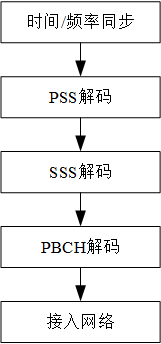
\includegraphics[scale=0.45]{fig5.eps}}
	%\caption{Distributed frequency synchronization process.}
	%\label{fig5}
	%\end{figure}
	
	\subsection{Clock Synchronization Mechanism Design}\label{CC}
	Clock synchronization schemes are mainly divided into two-way communication and broadcast schemes. The broadcast scheme uses the broadcast method to distribute the reference clock to all wireless nodes, which is usually used when the transmission delay is unstable and varies greatly.
	The 5G network itself has the characteristics of low latency and high stability, and in practical applications, the wireless network is mainly used for "last mile connection", and the distance to the same access point (AP) is usually much less than 100m, so the maximum propagation delay should be Less than 400ns, in view of this situation, for the sake of synchronization accuracy, the synchronization scheme is divided into two steps to execute:
	\begin{itemize}
		\item Determine the master-slave level of the wireless clock by broadcasting
		\item Pairwise two-way communication synchronization for nodes between adjacent levels
	\end{itemize}
	The wireless root node embeds the count k=0 into the synchronization message to broadcast and sends, and the received node sets the count k to k+1 as the local level and sends the broadcast synchronization message containing k+1 to the next level. And so on until all nodes have determined their level.
	The situation assumed in the research is a tree topology, and the binary tree is used for traversal. There is only broadcast communication between a single node and the left and right adjacent nodes, which is distributed layer by layer, as shown in the figure2:
	\begin{figure}[htbp]
		
		\centerline{\includegraphics[scale=0.5]{fig2.eps}}
		\caption{Wireless network clock synchronization topology, k represents the number of hops in the network, respectively.}
		\label{fig2}
	\end{figure}
	
	After the hierarchy level is established, synchronization is performed by a pairwise synchronization scheme, with each interval being one time slot.
	The slave clock will receive several reference timestamps G from the master clock through the middle, and record the local time L. 
	The algorithm for the synchronization process is as follows
	\begin{algorithm}[ht]  
		\caption{clock synchronization process in a clock level initialization period}  
		\begin{algorithmic}[1]
			\REQUIRE Time stamp sent by $k_{i-1}$ level clock, $T_G^n, n=1,2\ldots$; Local time stamp of $k$ level clock, $T_L^n,n=1,2\ldots$, clock synchronization period $ P_{sync}$, time slot \tau ; 
			\ENSURE corrected local clock, $L'$;
			
			\WHILE {$time \in P_{sync}$}
			\WHILE {$time = n\tau, n=1,2\ldots $}
			
			\IF {$State$ = initialization}
			\STATE $k_{i-1}$ level clock exchanges information with $k$ level clock, and $k$ level clock gets $T_G^n, n=1,2\ldots$;
			\IF {receives $T_G^n, n=1,2\ldots$}  
			\STATE record local time $T_L^n,n=1,2\ldots$, 
			\ENDIF
			\STATE the estimated values of frequency difference $\widehat{f}$ and clock deviation $\widehat{o}$ are obtained by linear regression;
			\STATE the $k_{i-1}$ level clock adjust its local time with $L' = L(1+\frac{\widehat{\sigma}}{f_0})-\widehat{o}+[\frac{G_0-L_0}{T_slot}]$;
			\ENDIF
			STATE=;
			\IF {receives $corr$}
			\STATE SM adjusts local time;
			\ENDIF
			\IF {$time+P_t>P_f$ \textbf{and} receives $f_{FM}$}
			\STATE SM adjusts local frequency;
			\ENDIF
			\ENDWHILE
			\ENDWHILE
			%\RETURN $T_{SM}'$.
		\end{algorithmic}
	\end{algorithm}
	After several groups of time stamps are exchanged, the estimated values of frequency difference and clock deviation are obtained by linear regression, and the local clock is corrected by the following formula:
	\begin{equation}
	L' = L(1+\frac{\widehat{\sigma}}{f_0})-\widehat{o}+[\frac{G_0-L_0}{T_slot}] \tag{2}
	\end{equation}
	It can be seen from the above formula that the influence caused by the accumulated error depends on the size of the time slot in the synchronization process, and the time slot determines the synchronization accuracy.
	The upper limit of accuracy, when the number of nodes increases, the synchronization delay increases, and the impact of the time slot length on the cumulative error is more obvious.
	\begin{equation}
	t=(\alpha +\sigma)t+\beta+\delta  \nonumber
	\end{equation}
	\begin{equation}
	t_(wired)=(\alpha _1+\sigma _1)t+\beta _1+\delta _1  \nonumber
	\end{equation}
	\begin{equation*}
	t_(wireless)=(\alpha _2+\sigma _2)t+\beta _2+\delta _2 \nonumber
	\end{equation*}
	\begin{equation}
	t_1=(\alpha _1+\sigma _1)t+\beta _1+\delta _1 \nonumber
	\end{equation}
	\begin{equation}
	t=\frac{t_1- \beta _1- \delta _1}{\alpha_1 + \sigma_1} \nonumber
	\end{equation}
	\begin{equation}
	t_2=(\frac{t_1- \beta _1- \delta _1}{\alpha_1 + \sigma_1}+delay)(\alpha_2+\sigma_2)+\beta_2+\delta_2 \nonumber
	\end{equation}
	\begin{equation}
	t=\frac{t_3-\beta_2-\delta_2}{\alpha_2+\sigma_2} \nonumber
	\end{equation}
	\begin{equation}
	t_4=(\frac{t_3-\beta_2-\delta_2}{\alpha_2+\sigma_2}+delay)(\alpha_1+\sigma_1)+\beta_1+\delta_1 \nonumber
	\end{equation}
	\begin{equation}
	m=\frac{\alpha_2+\sigma_2}{\alpha_1+\sigma_1} \nonumber
	\end{equation}
	\begin{equation}
	2delay=t_2-t_1+t_4-t_3 \nonumber
	\end{equation}
	\begin{equation}
	2delay=m(t_2-t_1+t_4-t_3)-(m-1/m)(\beta_1+\delta_1)+(m-1/m)(\beta_2+\delta_2) \nonumber
	\end{equation}
	\begin{equation}
	2delay=m(t_2-t_1+t_4-t_3)-(m-1/m)(\beta_2+\delta_2) \nonumber
	\end{equation}
	\begin{equation}
	2delay=m(t_2-t_1+t_4-t_3)-(m-1/m)(\beta_2+\delta_2) \nonumber
	\end{equation}
	\begin{equation}
	m=\frac{\alpha_2+\sigma_2}{\alpha_1+\sigma_2} \nonumber
	\end{equation}
	
	\subsection{Wireless end-to-end latency optimization}\label{CC}
	Since the research object is the wireless TSN network with 5G as the carrier, the 5G network frame structure is shown in the following figure:
	In 5G, the length of the radio frame and subframe is the same, the radio frame is 10ms, and the subframe length is 1ms
	The number of ofdm symbols contained in a time slot in 5G is 14, and the number of time slots contained in each subframe is different under different carrier intervals
	ssb (clock synchronization message) fixedly occupies 4 ofdm symbols, so the duration and period of ssb under different subcarrier intervals are different,
	The 5G subcarrier spacing is adjustable, and the 5G protocol has a recommended set of subcarrier spacing parameters for different application scenarios.
	Due to the assignable characteristics of the subcarrier spacing of the 5G network, the number of subcarriers can be reduced by increasing the subcarrier spacing, and the symbol length of the ofdm can be reduced, thereby reducing the delay and reducing the accumulated error.
	In the case of a certain transmission environment, the coherence bandwidth is the same, the larger the subcarrier spacing (ie subcarrier bandwidth), the smaller the number of subcarriers, and the larger the bandwidth of each subcarrier, resulting in the possibility of frequency selective attenuation. higher (occurs when the signal bandwidth is greater than the coherence bandwidth). Therefore, in the simulation, it is necessary to meet the delay requirement first and then use the equalizer to compensate to ensure the synchronization accuracy.
	
	
	\begin{algorithm}[ht]  
		\caption{CM clock synchronization process in a $P_f$ period}  
		\begin{algorithmic}[1]
			\REQUIRE Time information sent by GM, $T_{GM}$; Time information sent by SM, $T_{SM}'$; Local time information of CM $T_{CM}$; Frequency sent by FM, $f_{FM}$; Preset threshold, $\zeta$;
			\ENSURE Time correction value $corr$; GM status, $GS$;
			\WHILE {$time \in P_f$}
			\WHILE {receives $T_{SM}'$}
			\STATE CM calculates $corr$ and adjusts local time;  
			\STATE CM sends $corr$ to FM, SM and SC;
			\IF {$time+P_t>P_f$}
			\IF {receives $f_{FM}$}
			\STATE CM adjusts local frequency;
			\ENDIF
			\STATE $GS = abnormal$;
			\IF {receives $T_{GM}$ \textbf{and} $\left| T_{GM} - T_{CM}\right|  \le \zeta$}
			\STATE $GS = normal$;
			\ENDIF
			\ENDIF
			\ENDWHILE
			\ENDWHILE
			%\RETURN $corr$, $GS$.
		\end{algorithmic}
	\end{algorithm}
	
	
	\begin{algorithm}[ht]  
		\caption{FM clock synchronization process in a $P_f$ period}  
		\begin{algorithmic}[1]
			\REQUIRE Time information sent by GM, $T_{GM}'$; Time correction value sent by CM, $corr$; GM status, $GS$;
			\ENSURE Local frequency information of FM, $f_{FM}$;
			\WHILE {$time \in P_f$}
			\REPEAT
			\IF {$GS$ = normal}
			\IF {receives $T_{GM}'$}
			\STATE FM calculates frequency offset and adjusts local frequency;
			\ENDIF
			\IF {receives $corr$}
			\STATE FM adjusts local time;
			\ENDIF
			\ENDIF
			\UNTIL {$time+P_t>P_f$}
			\STATE FM generates $f_{FM}$ and injects it into the network;
			\ENDWHILE
			%\RETURN $f_{FM}$.
		\end{algorithmic}
	\end{algorithm}
	
	%The synchronization mechanism proposed in this paper combines tree-based and distributed synchronization. GM mainly provides an interface for the network to communicate with the external standard clock and synchronizes with SM. The underlying network clock reference is essentially a fault-tolerant mean provided by multiple SMs. Since all SMs are synchronized with GM, the clock reference of the underlying network is the same as GM and the calculation of the underlying network can eliminate the random errors caused during synchronization. Because the effect of the frequency offset is also taken into account during synchronization, the synchronization error will be smaller.
	
	%Once GM fails, the underlying network clock reference calculated by CM will be far away from the GM clock. Then the GM clock will be discarded, and the clock reference will directly adopt the clock value calculated by CM. Since SM has been synchronized with GM, the underlying clock reference and the actual clock of GM will not deviate significantly. So that even if a failure occurs, the reliability of the synchronization system can still be guaranteed.
	
	
	
	
	
	
	
	
	
	
	\section{Performance Evaluation}
	
	In this section, we investigate the effectiveness of our proposed hierarchical clock synchronization mechanism. A network structure was built in OMNET++ to verify the performance, as shown in Fig. 5. We first remodeled the clock in OMNET++ according to the mathematical model of the clock (1) and (2) established in section II. The frequency of GM is set to $1$MHz. Set the parameters of all other nodes to $\Delta_0=20$ppm, $F_i=1$MHz, $\delta=20$ppm, and $\phi_i \sim \mathcal N(0,{0.1}^2)$. We choose the SC node as the comparison node and set the bandwidth of all links to $100$M. The propagation delay of all links is set to $25$ns. Then the proposed mechanism is compared with the gPTP in terms of synchronization accuracy and speed.
	
	
	
	\subsection{Synchronization Accuracy}
	Fig. 6 shows the tendency of the synchronization errors over time when using the synchronization mechanism we proposed and gPTP with $P_t=2$s. From Fig. 6, one can see that the synchronization errors of gPTP produce large fluctuations due to the influence of frequency offset, and errors of our proposed mechanism change steadily. Under our proposed mechanism, the errors are lower than those under gPTP. The results imply the effectiveness of our mechanism. The frequency offset can cause cumulative time errors, resulting in poor performance. Our proposed mechanism synchronizes the frequency and eliminates errors caused by frequency offset.
	
	
	
	Fig. 7 shows the synchronization errors that our proposed mechanism and gPTP can achieve with different $ P_t $. The box plot in the figure is the synchronization errors obtained with the increase of simulation time in each period. The line in the figure and the small graph are the medians of the synchronization errors obtained with different $ P_t $. We can see that with the same $P_t$, the errors of the proposed mechanism is smaller than that of gPTP, which means our proposed mechanism can maintain high synchronization accuracy. As the $P_t$ decreases, this difference also decreases. This is because as $ P_t $ decreases, the errors caused by the frequency offset gradually decrease, and the gPTP errors also become smaller. Furthermore, from the box plot in the figure, we can see that the errors of the proposed mechanism are limited to a specific range, and the fluctuation is smaller, which is better than gPTP.
	
	
	
	\subsection{Synchronization Speed}
	Fig. 8 shows the synchronization speed of the two mechanisms with different $P_t$. We define the synchronization speed as the time when the relative error between the current synchronization accuracy and the median synchronization accuracy is $20\%$. It can be observed from the figure that the time required for our proposed mechanism is shorter than gPTP, which means that the synchronization speed of our proposed mechanism is faster and synchronization efficiency is higher than gPTP. The synchronization speed of gPTP is slow because it requires multiple cycles of synchronization to eliminate the errors gradually. Moreover, the frequency offset will continue to bring errors, resulting in a long time to achieve the required synchronization accuracy. Our method relies on the SM to provide a reference clock to eliminate errors at the beginning of synchronization quickly. After frequency synchronization, the errors become smaller, so that the synchronization accuracy is always kept in a low range.
	
	
	\subsection{Performance Analysis}
	The synchronization mechanism proposed in this work adopts a hierarchical structure. Since all SMs are synchronized with GM, the calculation of the underlying network can eliminate random errors. Moreover, due to the combination of distributed synchronization, which avoids the situation that tree-based synchronization errors will accumulate as the network scale increases, the synchronization process can be increased compared to gPTP with the same synchronization period. It can achieve the required synchronization accuracy faster, resulting in higher synchronization efficiency, which can also be seen from Fig. 8. 
	
	%\subsection{Reliability}
	%Fig. 9 shows the tendency of the synchronization accuracy of the two synchronization mechanisms under abnormal GM conditions. At the beginning of the figure, both mechanisms work normally. However, assuming that the GM is abnormal in the middle, we find that the synchronization accuracy of PTP will be severely affected later, but the synchronization mechanism proposed in this paper can still guarantee high synchronization accuracy. This is because we designed an exception judgment mechanism during synchronization to ensure the reliability of synchronization.
	
	\section{Conclusions}
	This paper has studied the clock synchronization for TSN. A hierarchical clock synchronization mechanism was proposed. Considering the synchronization time slot difference and the time-frequency coupling relationship, the offset of time and frequency are cooperatively regulated. Through the performance analysis and verification, the effectiveness and performance improvement of the proposed hierarchical synchronization mechanism was demonstrated. In the future, we will do further research on synchronization reliability.
	
	\section*{Acknowledgment}
	This work was supported  by National Key Research and Development Program of China (2018YFB1702100).
	
	%\begin{thebibliography}{00}
	%\bibitem{b1} G. Eason, B. Noble, and I. N. Sneddon, ``On certain integrals of Lipschitz-Hankel type involving products of Bessel functions,'' Phil. Trans. Roy. Soc. London, vol. A247, pp. 529--551, April 1955.
	%\bibitem{b2} J. Clerk Maxwell, A Treatise on Electricity and Magnetism, 3rd ed., vol. 2. Oxford: Clarendon, 1892, pp.68--73.
	%\bibitem{b3} I. S. Jacobs and C. P. Bean, ``Fine particles, thin films and exchange anisotropy,'' in Magnetism, vol. III, G. T. Rado and H. Suhl, Eds. New York: Academic, 1963, pp. 271--350.
	%\bibitem{b4} K. Elissa, ``Title of paper if known,'' unpublished.
	%\bibitem{b5} R. Nicole, ``Title of paper with only first word capitalized,'' J. Name Stand. Abbrev., in press.
	%\bibitem{b6} Y. Yorozu, M. Hirano, K. Oka, and Y. Tagawa, ``Electron spectroscopy studies on magneto-optical media and plastic substrate interface,'' IEEE Transl. J. Magn. Japan, vol. 2, pp. 740--741, August 1987 [Digests 9th Annual Conf. Magnetics Japan, p. 301, 1982].
	%\bibitem{b7} M. Young, The Technical Writer's Handbook. Mill Valley, CA: University Science, 1989.
	%\end{thebibliography}
	
	\bibliographystyle{IEEEtran}
	\bibliography{REF}
	
\end{document}